\chapter{Results}

\section{Goals}
We want to look at the effect that extending a KG has on the rules mined from it and the effect of different factors in the KG extension process. Will new correct rules be mined when the KG is extended with facts deemed plausible by a KG embedding? Are these new rules of the same quality as rules mined from the original KG. Will all the original rules also be mined from the extended KG? Furthermore we want to evaluate the effect of parameter choice when extending the KG, namely the KG embedding model architecture, the entity selection method and rank cutoff.

\section{Overview of results}

\subsection{KG extension sizes}
In the KG extension process there are 48 different parameter combinations. This means that there are 48 different KG extensions for each original KG. Extension set sizes ranged from around 800 to 33500 triples, where the RandomBaseline model admitted the most candidates. This makes sense, as the models assigns a random score to triples resulting in many more triples receiving a high rank. The other trained models give most candidates a low score because most triples are bad candidates. Note that the extension sizes were about the same for both datasets, while WN18RR and the family KG respectively have 88 227 and 258 235 facts, therefore the extensions for WN18RR are relatively larger than for the family KG.

\subsection{Rule set sizes and mean PCA confidence}
\label{TransE_sucks} 
When examining the number of rules mined in each KG extension one immediately sees some startling results. Most rule sets don't differ drastically in size apart from those where TransE was used, where these rule sets are exceptionally larger. See figure X and Y (TODO: add figures) in the appendix to observe the difference. When looking at the mean PCA confidence of the rules sets one also notes that the score for the TransE sets are mostly around 0.1, while the remaining rule sets have a score on average around 0.5.

\begin{figure}[h]
\centering
\begin{subfigure}{.5\textwidth}
  \centering
  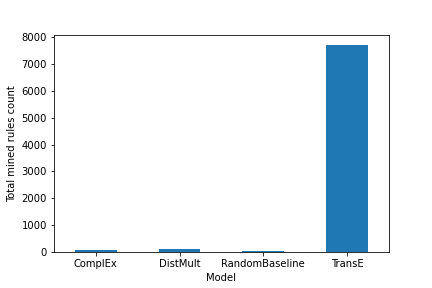
\includegraphics[width=1\linewidth]{figures/results/Total_mined_rules-model-wn18rr.png}
  \caption{WN18RR}
  \label{fig:sub1}
\end{subfigure}%
\begin{subfigure}{.5\textwidth}
  \centering
  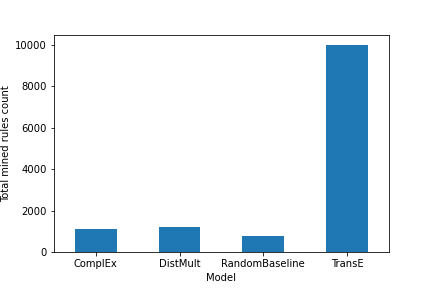
\includegraphics[width=1\linewidth]{figures/results/Total_mined_rules-model-family.png}
  \caption{Family KG}
  \label{fig:sub2}
\end{subfigure}
\caption{Distribution of number of mined rules over different embedding models.}
\label{fig:test}
\end{figure}

As discussed in (TODO: add section) TransE is not able to learn some type of relations, and upon further inspection of the embedding vectors for relations in TransE the vector values all tend toward zero. It seems that while scoring decently on the performance metrics during model selection, TransE has not properly embedded the relations in the KG. Of the rules mined, 97\% (WN18RR) and 76\% (family KG) come from KGs extended using TransE. Due to the fact that the trained TransE model has poor relational embeddings and that the large number of rules produced from this overshadow the rules mined using other embedding models, we will include  rules mined from KGs when examining embedding models, but not consider these data points when looking at entity selection methods or rank cutoff criteria.

\section{Effect of parameters}
In this section we will examine the effects of each parameter, namely the choice of KG embedding model, the choice of entity selection strategy and rank cutoff value. Note that when looking at rules mined with a certain parameter the sets of rules will be a concatenation of all cases where that parameter was in use. For example, if we look at the rules mined with ComplEx as the KG embedding model, then this group will contain rules mined from 12 different KG extensions because we need to look at all the combinations of entity selection methods and rank cutoff values ($4\times3=12$). This is differentiated from the case where we look at rules mined from a single extended KG, which we will do in section (TODO: add section).

\subsection{Effect of KG embedding model}
At the first glance of figures \ref{fig:model_pies_family} and \ref{fig:model_pies_wn18rr} it may seem odd that the PCA confidence of rules mined from RandomBaseline extensions is so high. By looking at figures (TODO: add hbar figs) and (TODO: add) it becomes apparent that there in fact fewer different rules mined from these extensions. In the WN18RR case no new rules were found, and one original rule was also never mined. The omitted rule,
\[derivationally\_related\_form(x, y)   \Rightarrow derivationally\_related\_form(y, x)\]
has the lowest PCA confidence out of all the original rules. Since there already was little support in the KG for the rule the addition of noise must have obscured too much evidence of \texttt{derivationally\_related\_form} being reflexive for AMIE3 to pick up on it. The family KG produced similar results, where AMIE3 failed to find 12 original rules in the RandomBaseline-extended KGs. All of these rules were among those with the lowest PCA confidence of the original rules.
Since the introduction of noise leads to the rules with lower PCA confidence to be removed it explains how the rules mined from RandomBaseline-extended KGs have a higher median PCA confidence than the original rules, as seen in figures \ref{fig:model_pies_family} and \ref{fig:model_pies_wn18rr}.

\begin{figure}[h]
\centering
\begin{subfigure}{.5\textwidth}
  \centering
  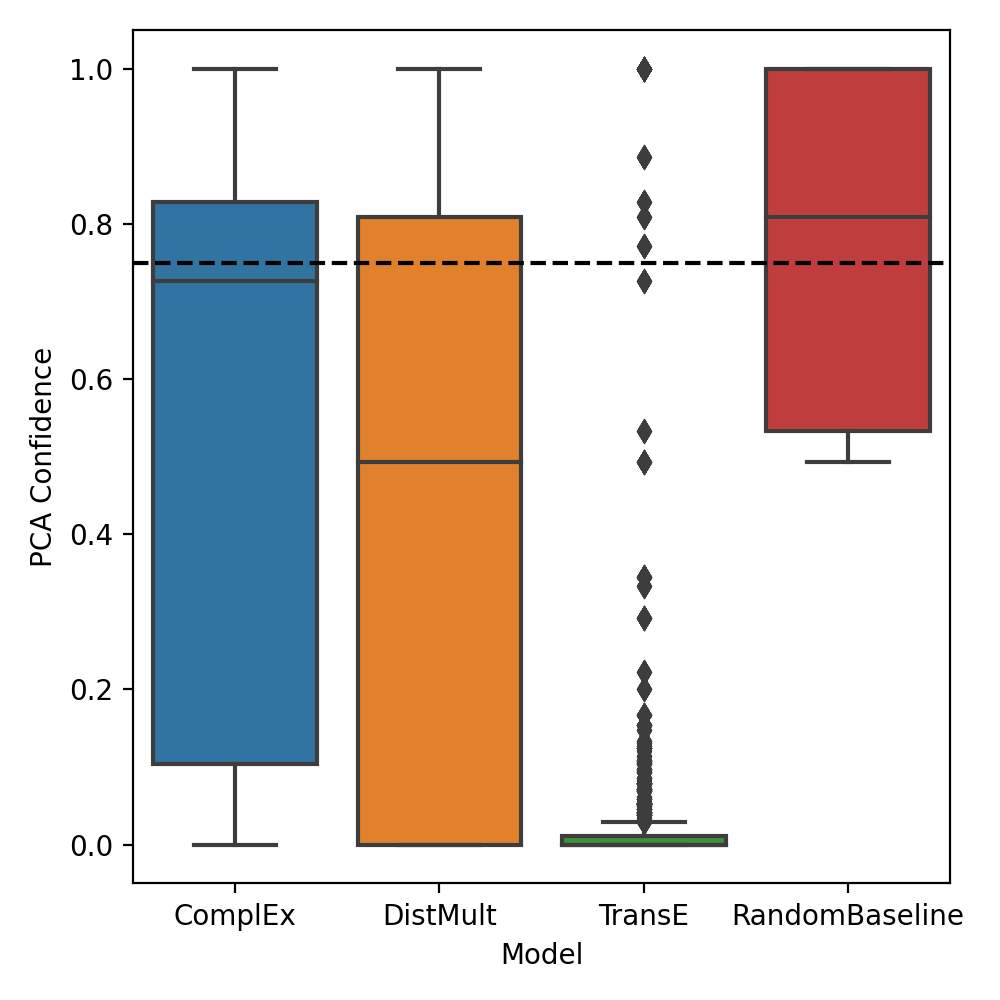
\includegraphics[width=1\linewidth]{figures/results/PCA_models/PCA-models_wn18rr.png}
  \caption{Original KG}
  \label{fig:PCA-models_wn18rr_boxplot_sub}
\end{subfigure}%
\begin{subfigure}{.5\textwidth}
  \centering
  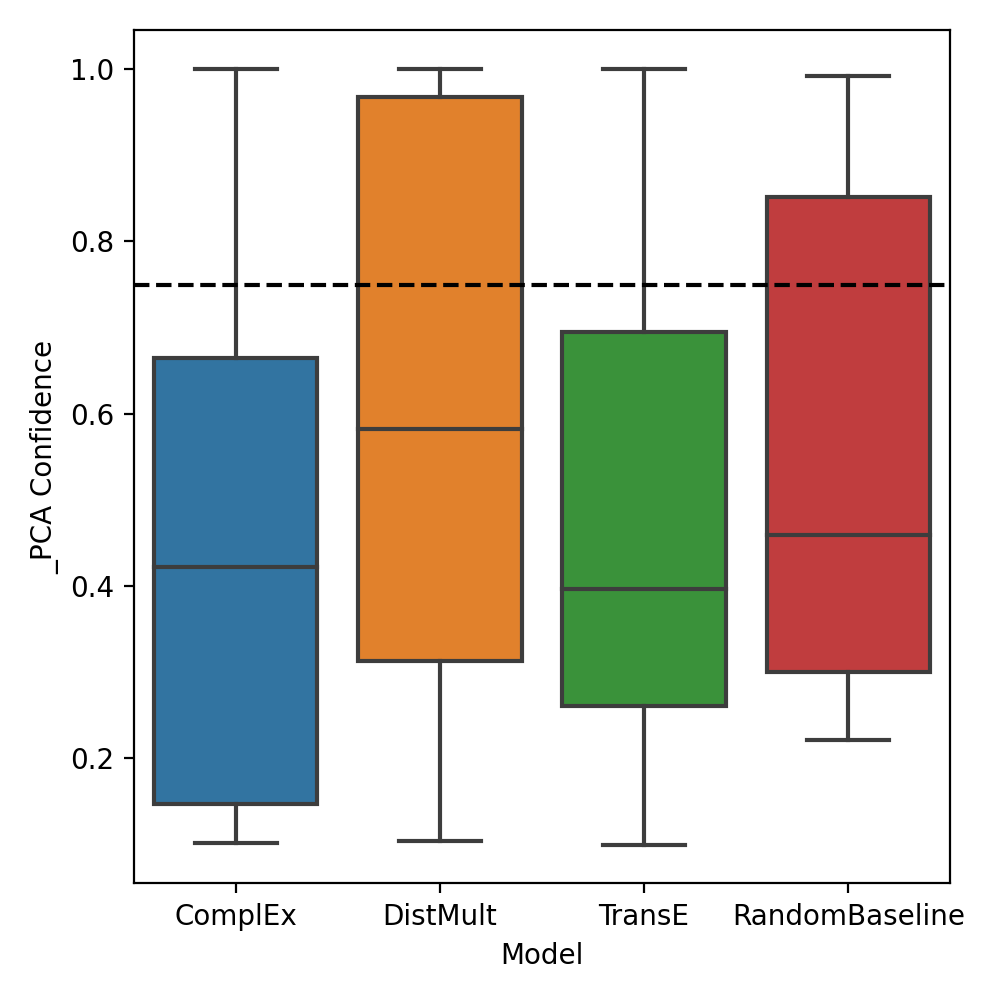
\includegraphics[width=1\linewidth]{figures/results/PCA_models/_PCA-models_wn18rr.png}
  \caption{Extended KG}
  \label{fig:_PCA_models_wn18rr_boxplot_sub}
\end{subfigure}
\caption{Distribution of PCA confidence of mined rules by KG embedding models. PCA confidence scores are calculated on the original WN18RR and the extended WN18RR from which the rules are mined. The dashed line represents the median PCA confidence of the rules mined from the original WN18RR KG.}
\label{fig:PCA_models_wn18rr_boxplot}
\end{figure}

\begin{figure}[h]
\centering
\begin{subfigure}{.5\textwidth}
  \centering
  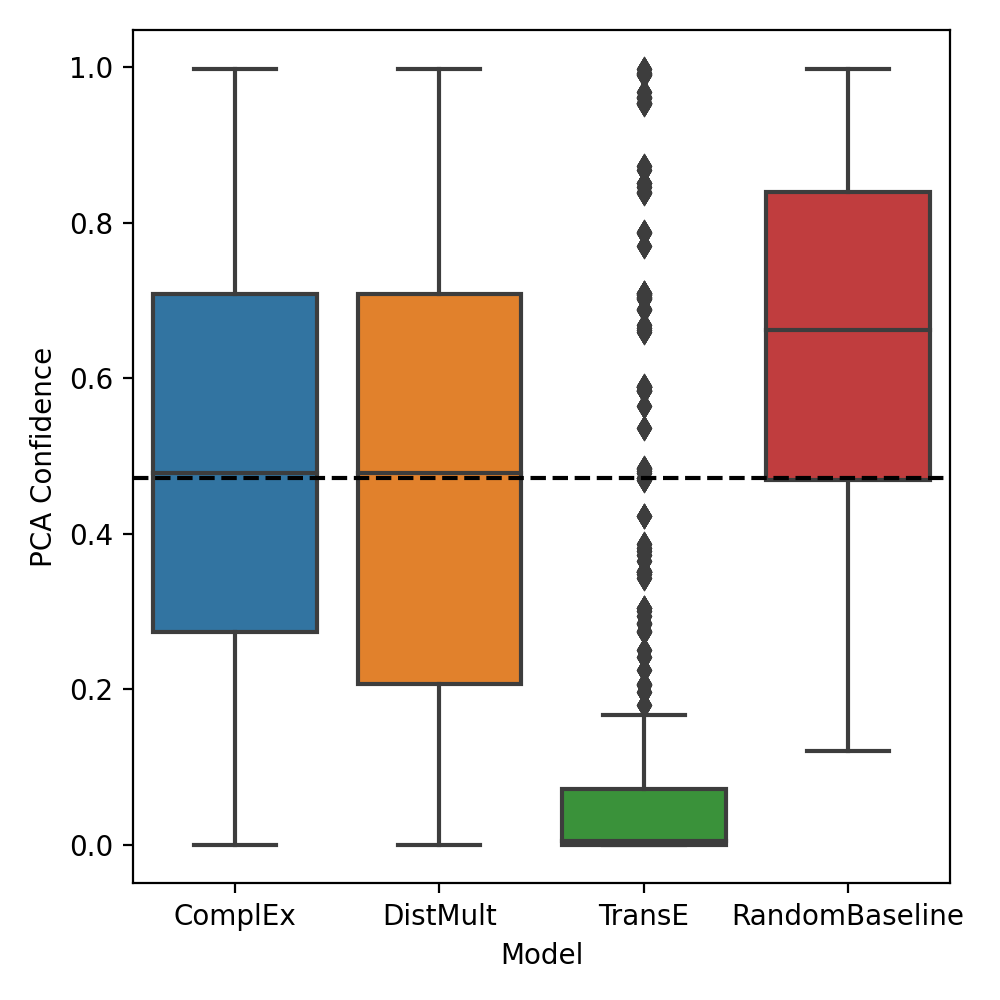
\includegraphics[width=1\linewidth]{figures/results/PCA_models/PCA-models_family.png}
  \caption{Original KG}
  \label{fig:models_family_boxplot_sub}
\end{subfigure}%
\begin{subfigure}{.5\textwidth}
  \centering
  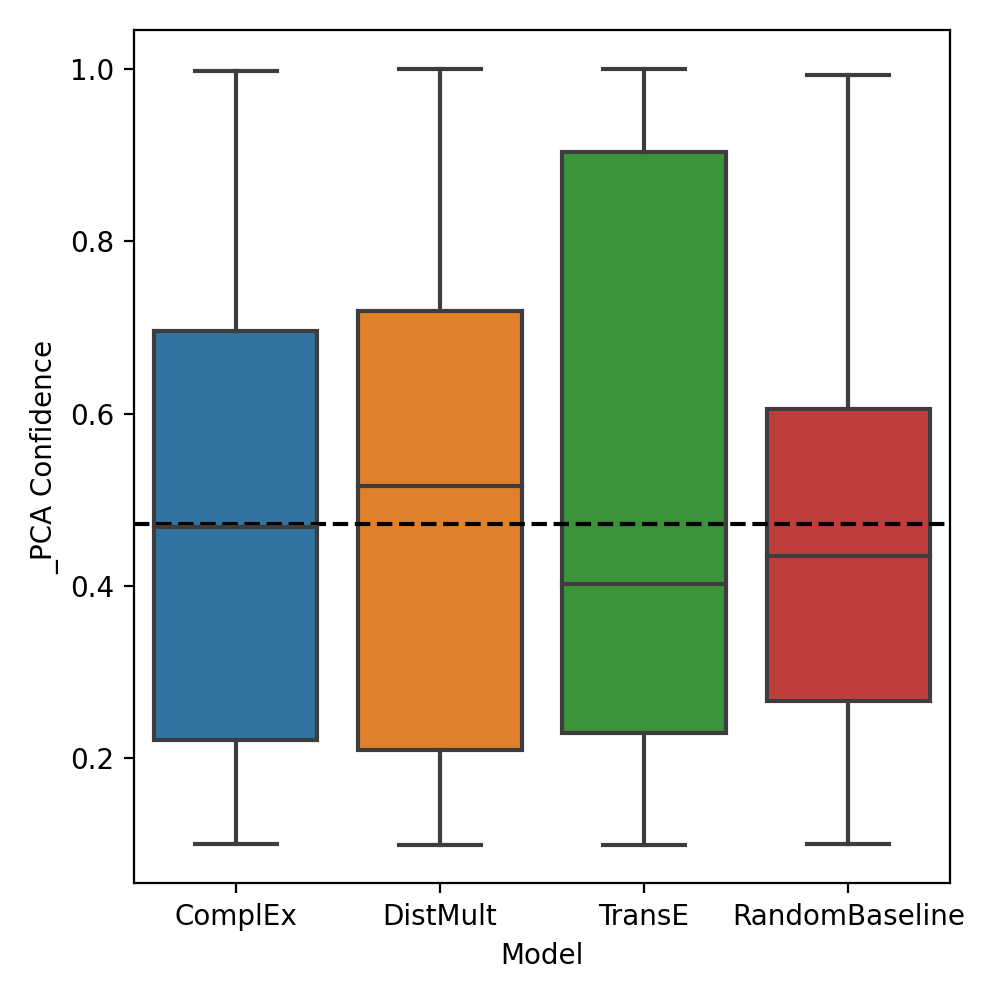
\includegraphics[width=1\linewidth]{figures/results/PCA_models/_PCA-models_family.png}
  \caption{Extended KG}
  \label{fig:_PCA_models_family_boxplot_sub}
\end{subfigure}
\caption{Distribution of PCA confidence of mined rules by KG embedding models. PCA confidence scores are calculated on the original family KG and the extended family KG from which the rules are mined. The dashed line represents the median PCA confidence of the rules mined from the original family KG.}
\label{fig:PCA_models_family_boxplot}
\end{figure}


As presented in \cref{TransE_sucks}, AMIE3 mines a lot more rules from KGs extended with TransE. Of the new rules mined 99\% (family KG) and 76\% (WN18RR) of the rules mined are mined from these KGs. Due to the low mean PCA confidence for these rules (0.038 for WN18RR and 0.089 for the family KG) it is clear that there is little support for the rules in the original KGs. If one however evalates the TransE rules on the extended KGs they were mined from, the PCA confidence increases by a lot, as seen in figures \ref{fig:model_pies_family} and \ref{fig:model_pies_wn18rr}. So even though most of the rules have little support from the original KGs, it was no mistake that AMIE3 mined so many rules from the TransE-extended KGs.

\begin{table}[h]
\begin{tabular}{|l|ccc||ccc|}
\hline
{\textbf{DATASET}}   & \multicolumn{3}{c||}{\textbf{WN18RR}}                                                                              & \multicolumn{3}{c|}{\textbf{Family KG}}                                                           \\ \hline
{\textbf{RULE GROUPS}}   & \multicolumn{1}{c|}{\textbf{Not found}} & \multicolumn{1}{c|}{\textbf{Found}} & \multicolumn{1}{c||}{\textbf{New}} & \multicolumn{1}{c|}{\textbf{Not found}} & \multicolumn{1}{c|}{\textbf{Found}} & \multicolumn{1}{c|}{\textbf{New}} \\ \hline
\textbf{ComplEx}  & \multicolumn{1}{c|}{0}                  & \multicolumn{1}{c|}{10}             & \multicolumn{1}{c||}{19}           & \multicolumn{1}{c|}{0}                  & \multicolumn{1}{c|}{94}             & \multicolumn{1}{c|}{73}           \\ \hline
\textbf{DistMult} & \multicolumn{1}{c|}{0}                     & \multicolumn{1}{c|}{10}                                  & 16                                & \multicolumn{1}{c|}{1}         & \multicolumn{1}{c|}{93}          & 115                               \\ \hline
\textbf{TransE}   & \multicolumn{1}{c|}{0}         & \multicolumn{1}{c|}{10}                     & 811                               & \multicolumn{1}{c|}{7}       & \multicolumn{1}{c|}{87}      & 1083                              \\ \hline
\textbf{Baseline} & \multicolumn{1}{c|}{1}     & \multicolumn{1}{c|}{9}                   & 0                                 & \multicolumn{1}{c|}{12}       & \multicolumn{1}{c|}{82}         & 16                                \\ \hline
\end{tabular}
\caption{Overview of which KG embedding models found all the original rules and how many new rules were found.}
\end{table}

DistMult and ComplEx are relatively similar embedding models as they have similar scoring functions (the scoring function of ComplEx corresponds to that of DistMult but with real embeddings), and perform similarly on benchmark datasets \cite{complEx}. As mentioned in section (TODO add section), DistMult is not able to learn asymmetry nor antisymmetry qualities to relations, however the type of rules AMIE3 can mine are not able to represent this either (TODO: add source or explanation). From the results it seems that ComplEx is a somewhat stricter model, in the sense that it ranks canidate triples lower against corrupted triples. THis is evidenced by the fact that the KG extensions sizes are larger for DistMult than ComplEx; DistMult is admitting more candidates. For example on the out of the candidates generated with the the entity selection method "probabillistic" from the WN18RR KG, DistMult assigned 1468 candidates rank 1 while ComplEx only did this for 866 candidates. As a result, more rules are mined from DistMult-extended KGs, as can be seen in (TODO: add fig). 

The combined set of rules found from ComplEx-extended KGs include all the original rules, both for WN18RR and the family KG.  This is almost also the case for DistMult, but it fails to find the original rule $child(x, y) \Rightarrow mother(y,x)$ in the family KG. This rule has the second lowest PCA confidence of all the original family KG rules.


TODO( correlations between rules mined from ComplEx and DistMult)


    \begin{figure*}[h]
        \centering
        \begin{subfigure}[b]{0.49\textwidth}
            \centering
            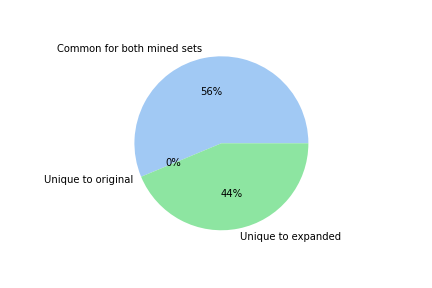
\includegraphics[width=\textwidth]{figures/results/pie_charts-model/complEx_family.png}
            \caption[complEx_pie]%
            {{\small ComplEx}}    
            \label{fig:complex_pie_family}
        \end{subfigure}
        \hfill
        \begin{subfigure}[b]{0.49\textwidth}  
            \centering 
            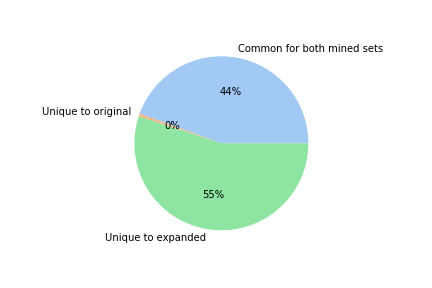
\includegraphics[width=\textwidth]{figures/results/pie_charts-model/distMult_family.png}
            \caption[]%
            {{\small DistMult}}    
            \label{fig:distMult_pie_family}
        \end{subfigure}
        \vskip\baselineskip
        \begin{subfigure}[b]{0.49\textwidth}   
            \centering 
            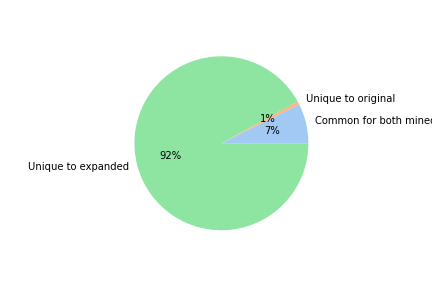
\includegraphics[width=\textwidth]{figures/results/pie_charts-model/transE_family.png}
            \caption[]%
            {{\small TransE}}    
            \label{fig:trasE_pie_family}
        \end{subfigure}
        \hfill
        \begin{subfigure}[b]{0.49\textwidth}   
            \centering 
            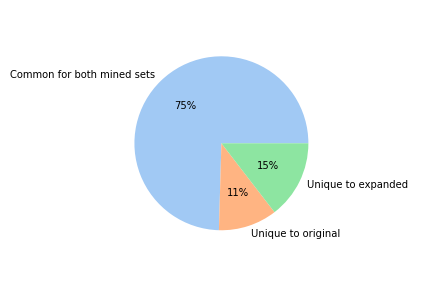
\includegraphics[width=\textwidth]{figures/results/pie_charts-model/randomBaseline_family.png}
            \caption[]%
            {{\small RandomBaseline}}    
            \label{fig:randomBaseline_pie_family}
        \end{subfigure}
        \caption[ The average and standard deviation of critical parameters ]
        {\small Distribution of all the rules mined over KG embedding models. KG: family KG.} 
        \label{fig:model_pies_family}
    \end{figure*}
    
    
    \begin{figure*}[h]
        \centering
        \begin{subfigure}[b]{0.49\textwidth}
            \centering
            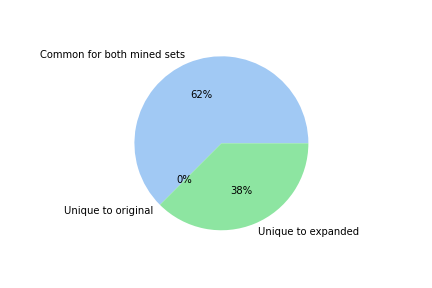
\includegraphics[width=\textwidth]{figures/results/pie_charts-model/complEx_wn18rr.png}
            \caption[complEx_pie]%
            {{\small ComplEx}}    
            \label{fig:complex_pie_wn18rr}
        \end{subfigure}
        \hfill
        \begin{subfigure}[b]{0.49\textwidth}  
            \centering 
            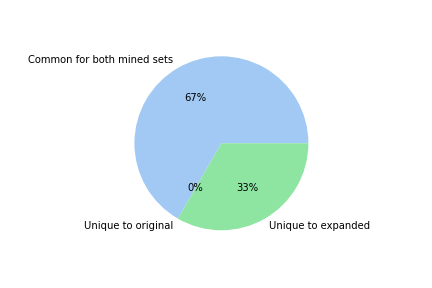
\includegraphics[width=\textwidth]{figures/results/pie_charts-model/distMult_wn18rr.png}
            \caption[]%
            {{\small DistMult}}    
            \label{fig:distMult_pie_wn18rr}
        \end{subfigure}
        \vskip\baselineskip
        \begin{subfigure}[b]{0.49\textwidth}   
            \centering 
            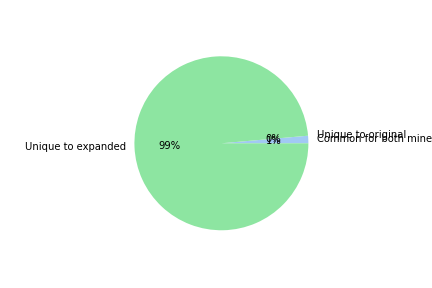
\includegraphics[width=\textwidth]{figures/results/pie_charts-model/transE_wn18rr.png}
            \caption[]%
            {{\small TransE}}    
            \label{fig:trasE_pie_wn18rr}
        \end{subfigure}
        \hfill
        \begin{subfigure}[b]{0.49\textwidth}   
            \centering 
            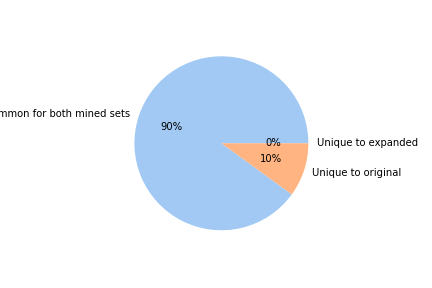
\includegraphics[width=\textwidth]{figures/results/pie_charts-model/randomBaseline_wn18rr.png}
            \caption[]%
            {{\small RandomBaseline}}    
            \label{fig:randomBaseline_pie_wn18rr}
        \end{subfigure}
        \caption[ The average and standard deviation of critical parameters ]
        {\small Distribution of all the rules mined over KG embedding models. KG: WN18RR.} 
        \label{fig:model_pies_wn18rr}
    \end{figure*}



\newpage
\subsection{Effect of entity selection method}
The \textit{probabilistic}, \textit{random}, and the \textit{least frequent} entity selection strategies perform relatively similarly if we look at the PCA confidence box plots in figures \ref{fig:PCA_entity_wn18rr_boxplot} and \ref{fig:PCA_entity_family_boxplot}. The \textit{most frequent} strategy, however, performs worse, both on the WN18RR and family KG. This is consistent with AmpliGraph's assumption that the most frequent entities are less likely to have missing facts.

In the WN18RR KG all original rules were found, but in the family KG only the \textit{least frequent} strategy resulted in all the original rules being mined. It also resulted in the least new rules being mined, while the\textit{most frequent} strategy led to the most new rules.

Overall it seems like \textit{probabilistic}, \textit{random}, and the \textit{least frequent} entity selection strategies all are appropriate entity selection strategies in regard to maintaining PCA confidence. If however the goal is to mine many new rules then \textit{most frequent} seems the most appropriate, though at the sacrifice of PCA confidence.

\begin{figure}[h]
\centering
\begin{subfigure}{.5\textwidth}
  \centering
  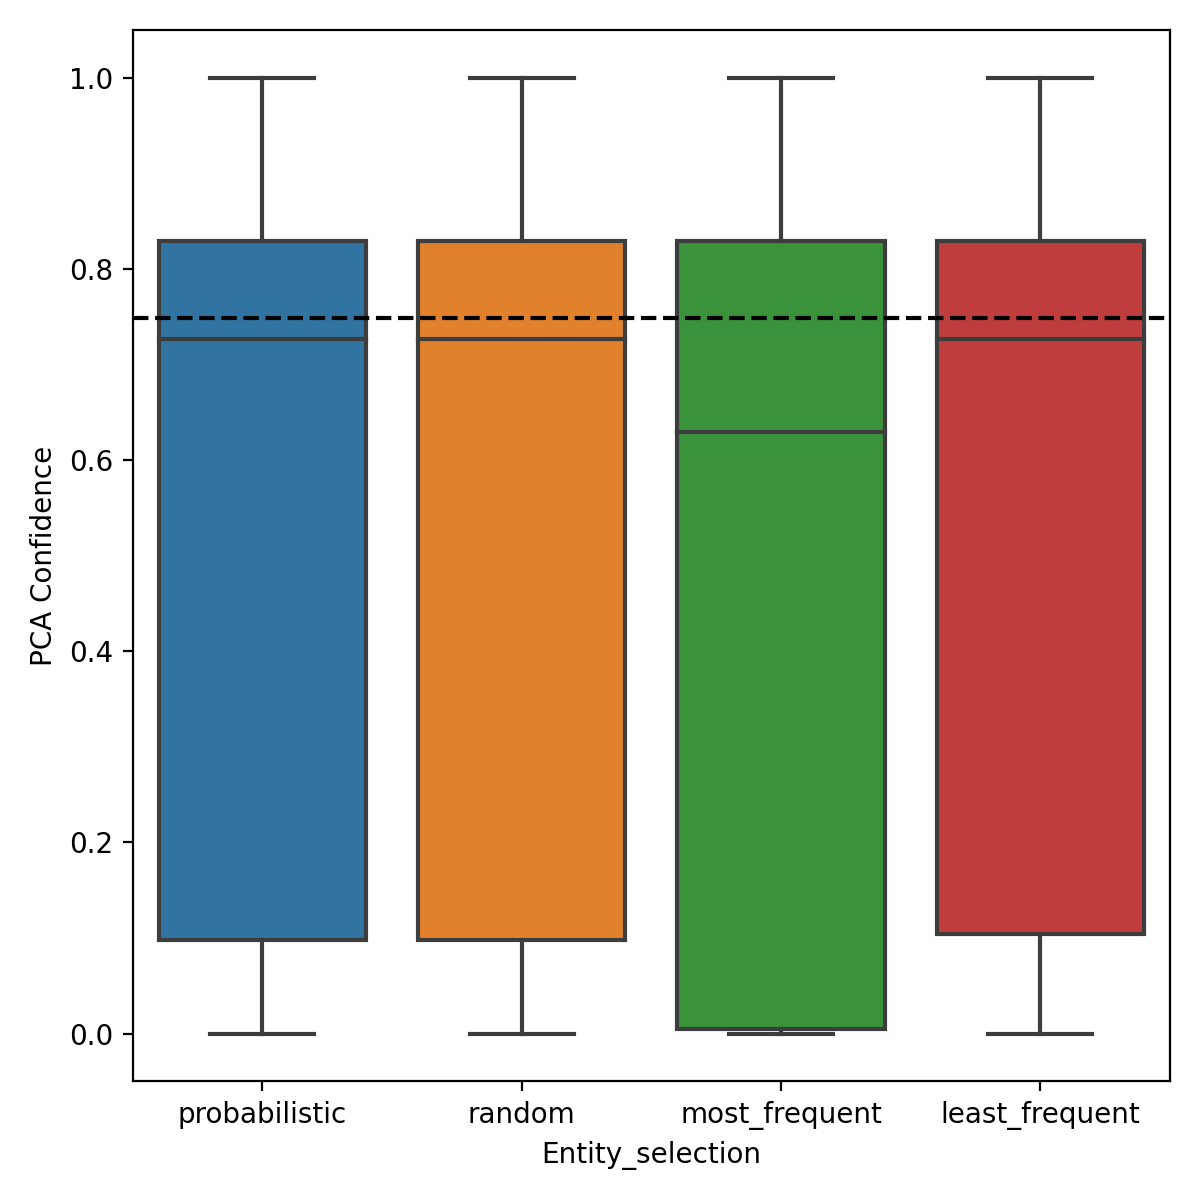
\includegraphics[width=1\linewidth]{figures/results/entity_selection/PCA-entity_wn18rr.png}
  \caption{Original KG}
  \label{fig:PCA-entity_wn18rr_boxplot_sub}
\end{subfigure}%
\begin{subfigure}{.5\textwidth}
  \centering
  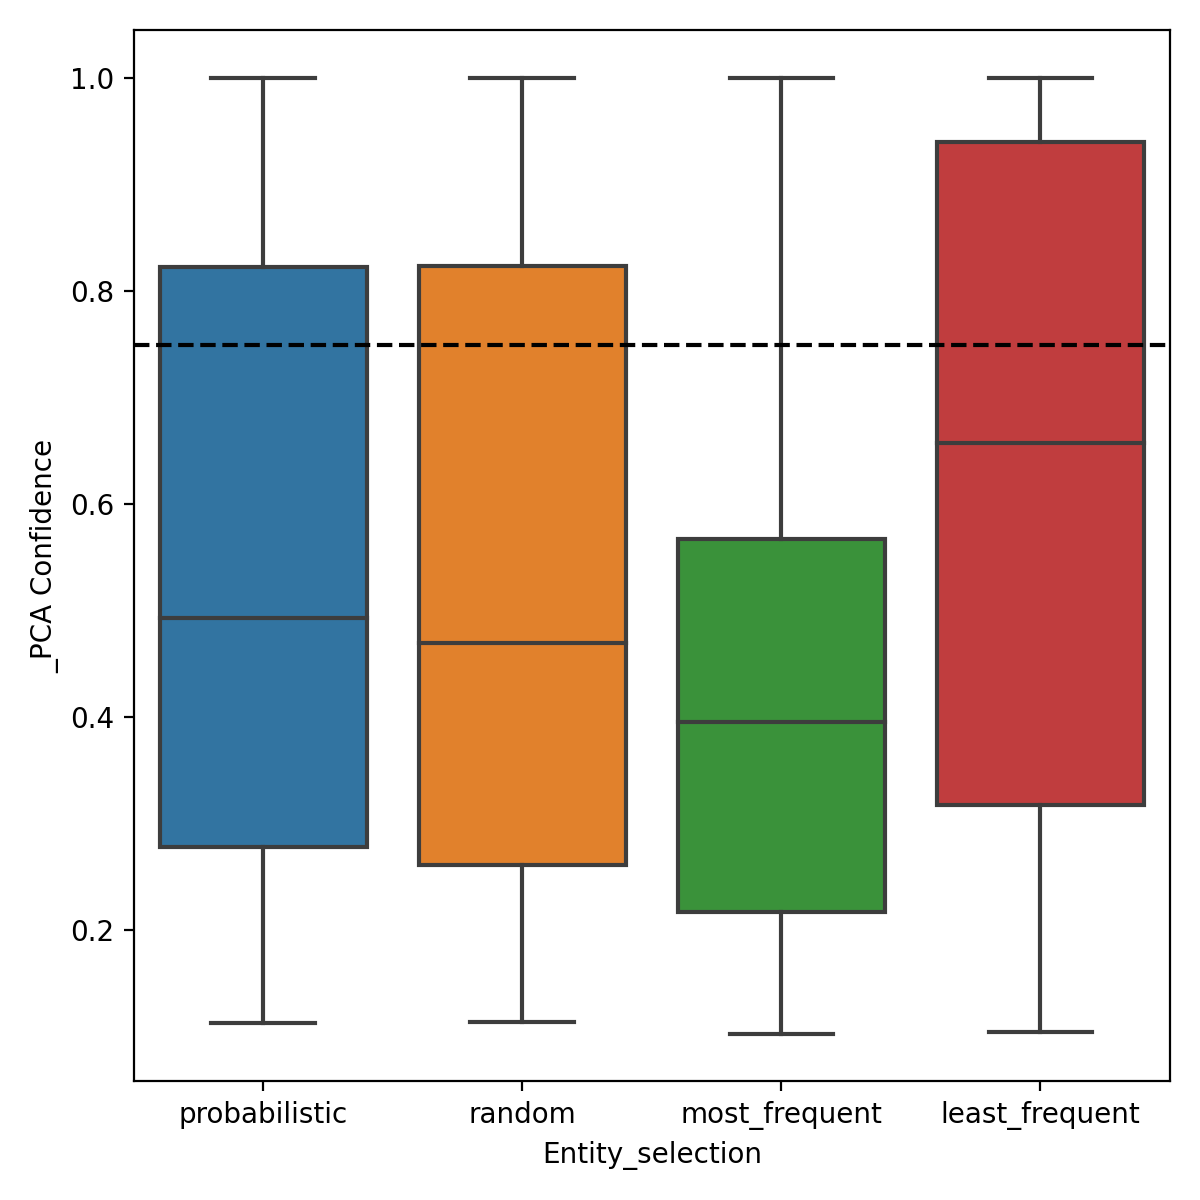
\includegraphics[width=1\linewidth]{figures/results/entity_selection/_PCA-entity_wn18rr.png}
  \caption{Extended KG}
  \label{fig:_PCA_entity_wn18rr_boxplot_sub}
\end{subfigure}
\caption{Distribution of PCA confidence of mined rules by entity selection strategies. PCA confidence scores are calculated on the original WN18RR and the extended WN18RR from which the rules are mined. The dashed line represents the median PCA confidence of the rules mined from the original WN18RR KG.}
\label{fig:PCA_entity_wn18rr_boxplot}
\end{figure}

\begin{figure}[h]
\centering
\begin{subfigure}{.5\textwidth}
  \centering
  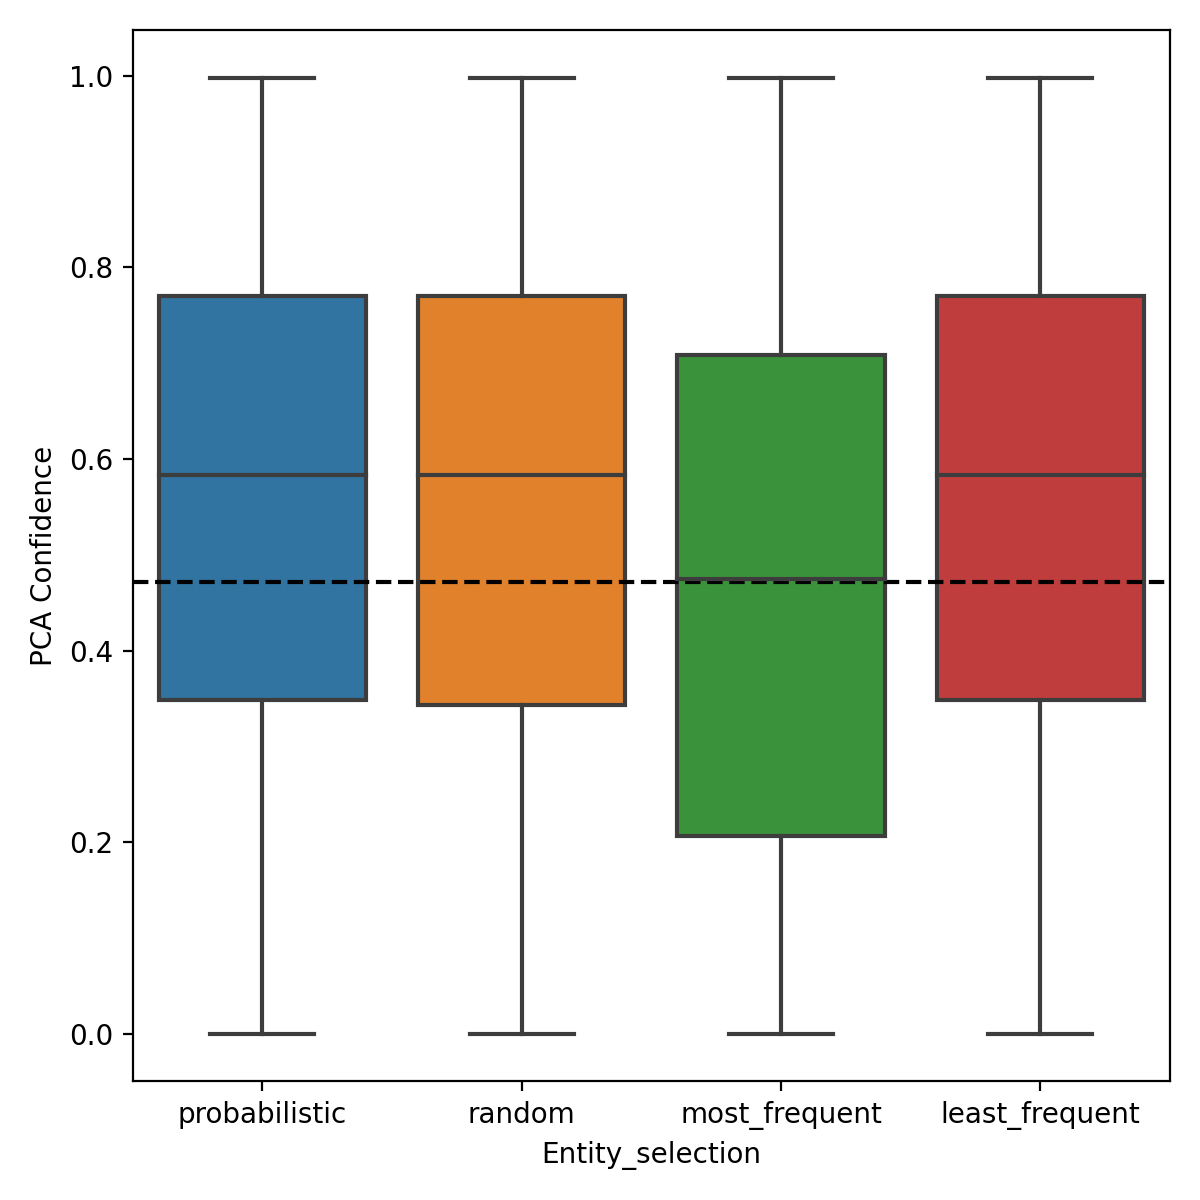
\includegraphics[width=1\linewidth]{figures/results/entity_selection/PCA-entity_family.png}
  \caption{Original KG}
  \label{fig:models_entity_boxplot_sub}
\end{subfigure}%
\begin{subfigure}{.5\textwidth}
  \centering
  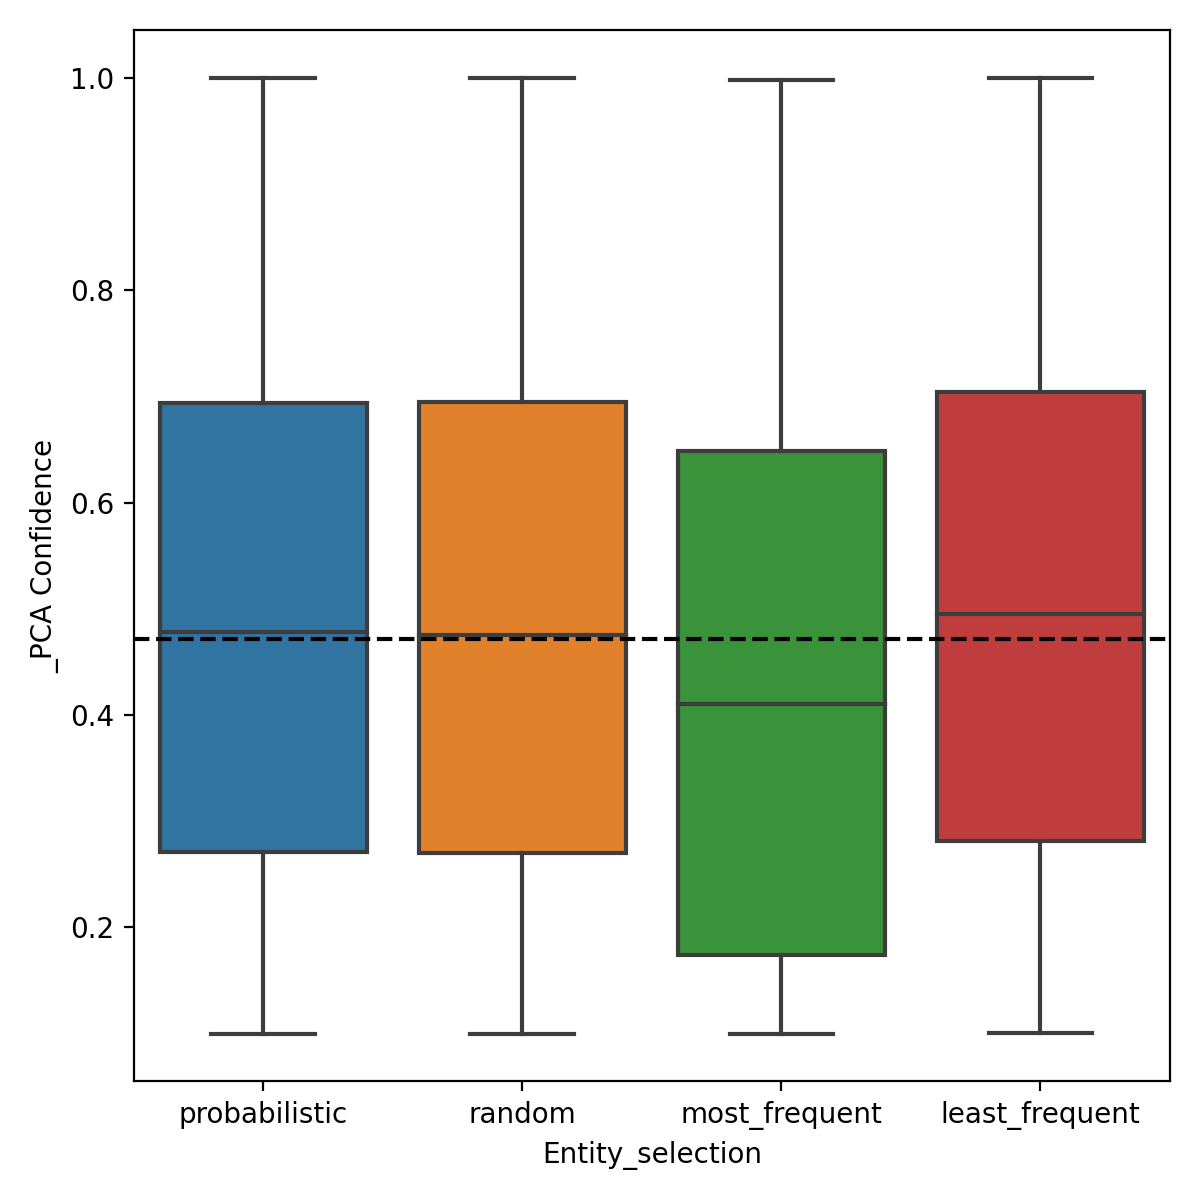
\includegraphics[width=1\linewidth]{figures/results/entity_selection/_PCA-entity_family.png}
  \caption{Extended KG}
  \label{fig:_PCA_entity_family_boxplot_sub}
\end{subfigure}
\caption{Distribution of PCA confidence of mined rules by entity selection strategies. PCA confidence scores are calculated on the original family KG and the extended family KG from which the rules are mined. The dashed line represents the median PCA confidence of the rules mined from the original family KG.}
\label{fig:PCA_entity_family_boxplot}
\end{figure}



\begin{figure*}[h]
        \centering
        \begin{subfigure}[b]{0.49\textwidth}
            \centering
            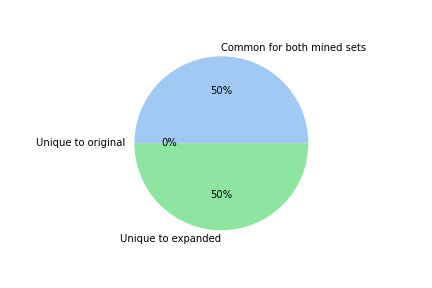
\includegraphics[width=\textwidth]{figures/results/entity_selection/pie_charts/probabilistic_wn18rr.png}
            \caption[complEx_pie]%
            {{\small Probabilistic}}    
            \label{fig:probabilistic_pie_wn18rr}
        \end{subfigure}
        \hfill
        \begin{subfigure}[b]{0.49\textwidth}  
            \centering 
            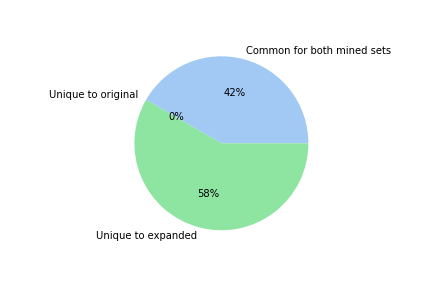
\includegraphics[width=\textwidth]{figures/results/entity_selection/pie_charts/random_wn18rr.png}
            \caption[]%
            {{\small Random}}    
            \label{random_pie_wn18rr}
        \end{subfigure}
        \vskip\baselineskip
        \begin{subfigure}[b]{0.49\textwidth}   
            \centering 
            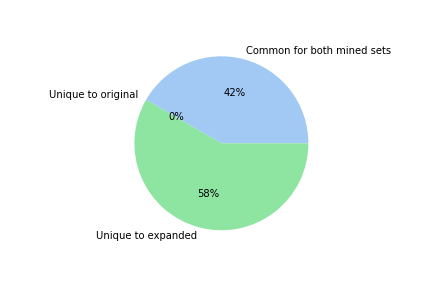
\includegraphics[width=\textwidth]{figures/results/entity_selection/pie_charts/most_frequent_wn18rr.png}
            \caption[]%
            {{\small Most Frequent}}    
            \label{fig:most_pie_wn18rr}
        \end{subfigure}
        \hfill
        \begin{subfigure}[b]{0.49\textwidth}   
            \centering 
            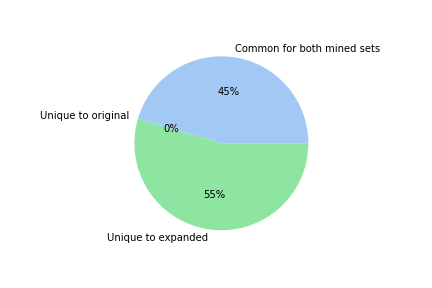
\includegraphics[width=\textwidth]{figures/results/entity_selection/pie_charts/least_frequent_wn18rr.png}
            \caption[]%
            {{\small Least Frequent}}    
            \label{fig:least_pie_wn18rr}
        \end{subfigure}
        \caption[]
        {\small Distribution of all the rules mined over entity selection stragegies for WN18RR.} 
        \label{fig:entity_pies_wn18rr}
    \end{figure*}
    
    
    \begin{figure*}[h]
        \centering
        \begin{subfigure}[b]{0.49\textwidth}
            \centering
            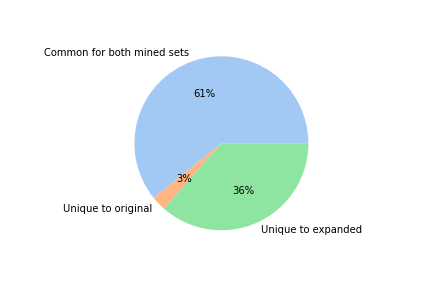
\includegraphics[width=\textwidth]{figures/results/entity_selection/pie_charts/Probabilistic_selection_family.png}
            \caption[]%
            {{\small Probabilistic}}    
            \label{fig:probablilistic_pie_family}
        \end{subfigure}
        \hfill
        \begin{subfigure}[b]{0.49\textwidth}  
            \centering 
            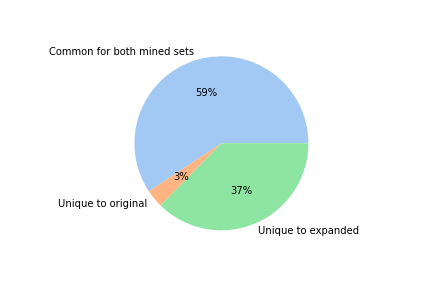
\includegraphics[width=\textwidth]{figures/results/entity_selection/pie_charts/random_family.png}
            \caption[]%
            {{\small Random}}    
            \label{fig:random_pie_family}
        \end{subfigure}
        \vskip\baselineskip
        \begin{subfigure}[b]{0.49\textwidth}   
            \centering 
            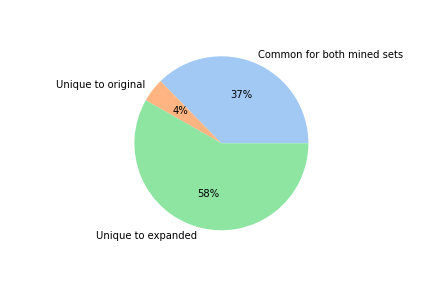
\includegraphics[width=\textwidth]{figures/results/entity_selection/pie_charts/most_frequent_family.png}
            \caption[]%
            {{\small Most Frequent}}    
            \label{fig:most_pie_family}
        \end{subfigure}
        \hfill
        \begin{subfigure}[b]{0.49\textwidth}   
            \centering 
            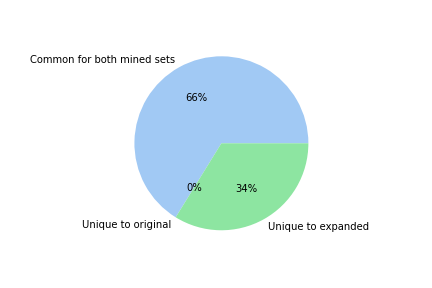
\includegraphics[width=\textwidth]{figures/results/entity_selection/pie_charts/least_frequent_family.png}
            \caption[]%
            {{\small Least Frequent}}    
            \label{fig:least_pie_family}
        \end{subfigure}
        \caption[]
        {\small Distribution of all the rules mined over entity selection strategies for the family KG.} 
        \label{fig:entity_pies_family}
    \end{figure*}






\newpage
\subsection{Effect of rank cutoff value}

\begin{figure}[h]
\centering
\begin{subfigure}{.5\textwidth}
  \centering
  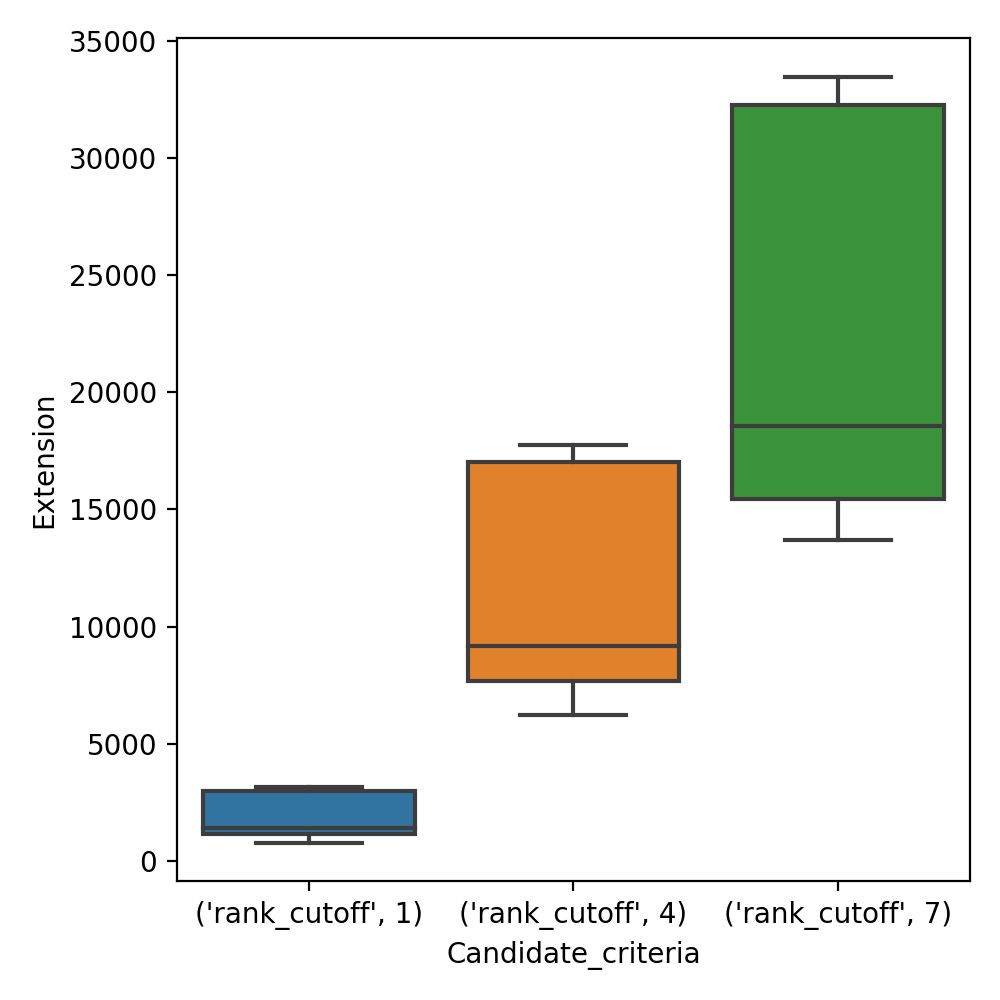
\includegraphics[width=1\linewidth]{figures/results/ranks/Extension_size_entity_wn18rr.png}
  \caption{WN18RR KG.}
  \label{fig:rank_extension_wn18rr_boxplot_sub}
\end{subfigure}%
\begin{subfigure}{.5\textwidth}
  \centering
  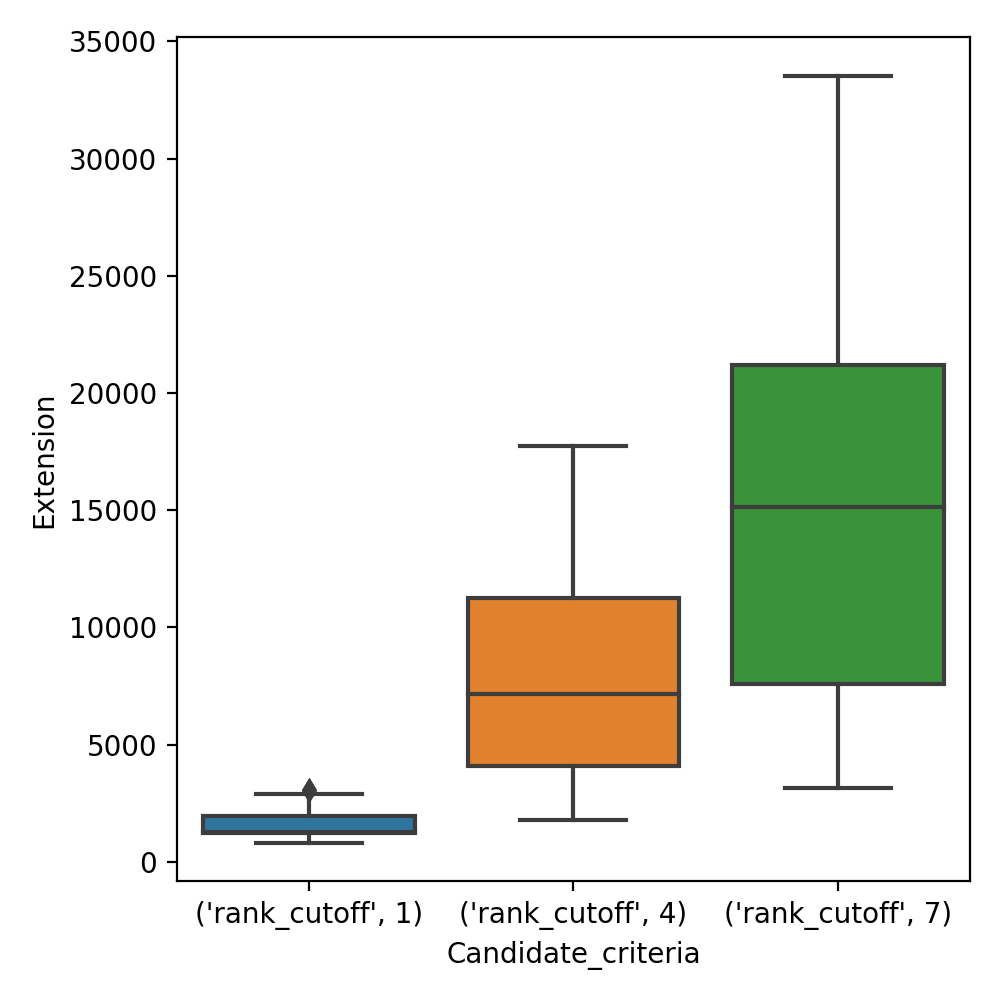
\includegraphics[width=1\linewidth]{figures/results/ranks/Extension_size_entity_family.png}
  \caption{Family KG.}
  \label{fig:rank_extension_family_boxplot_sub}
\end{subfigure}
\caption{Distribution of KG extension sizes over rank cutoff values.}
\label{fig:rank_extensions_boxplot}
\end{figure}

\begin{figure}[h]
\centering
\begin{subfigure}{.5\textwidth}
  \centering
  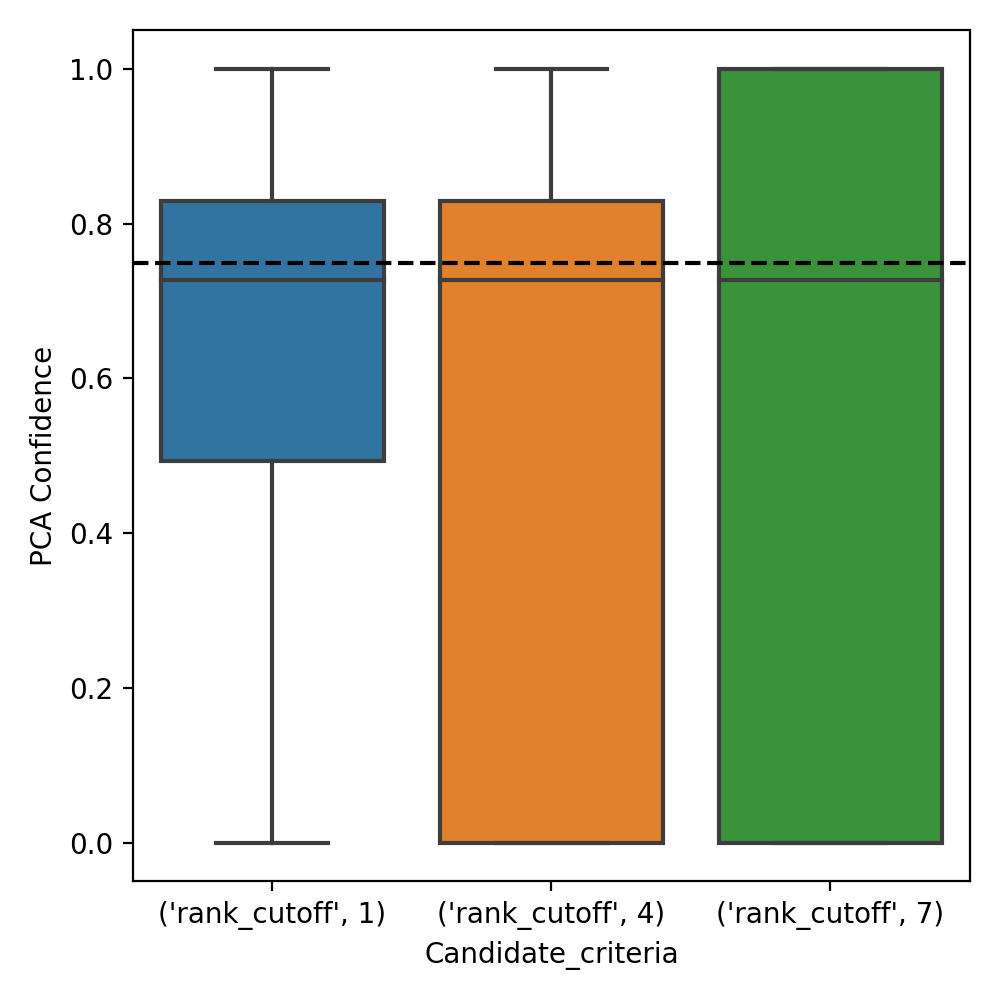
\includegraphics[width=1\linewidth]{figures/results/ranks/PCA-rank_wn18rr.png}
  \caption{Original KG}
  \label{fig:PCA-rank_wn18rr_boxplot_sub}
\end{subfigure}%
\begin{subfigure}{.5\textwidth}
  \centering
  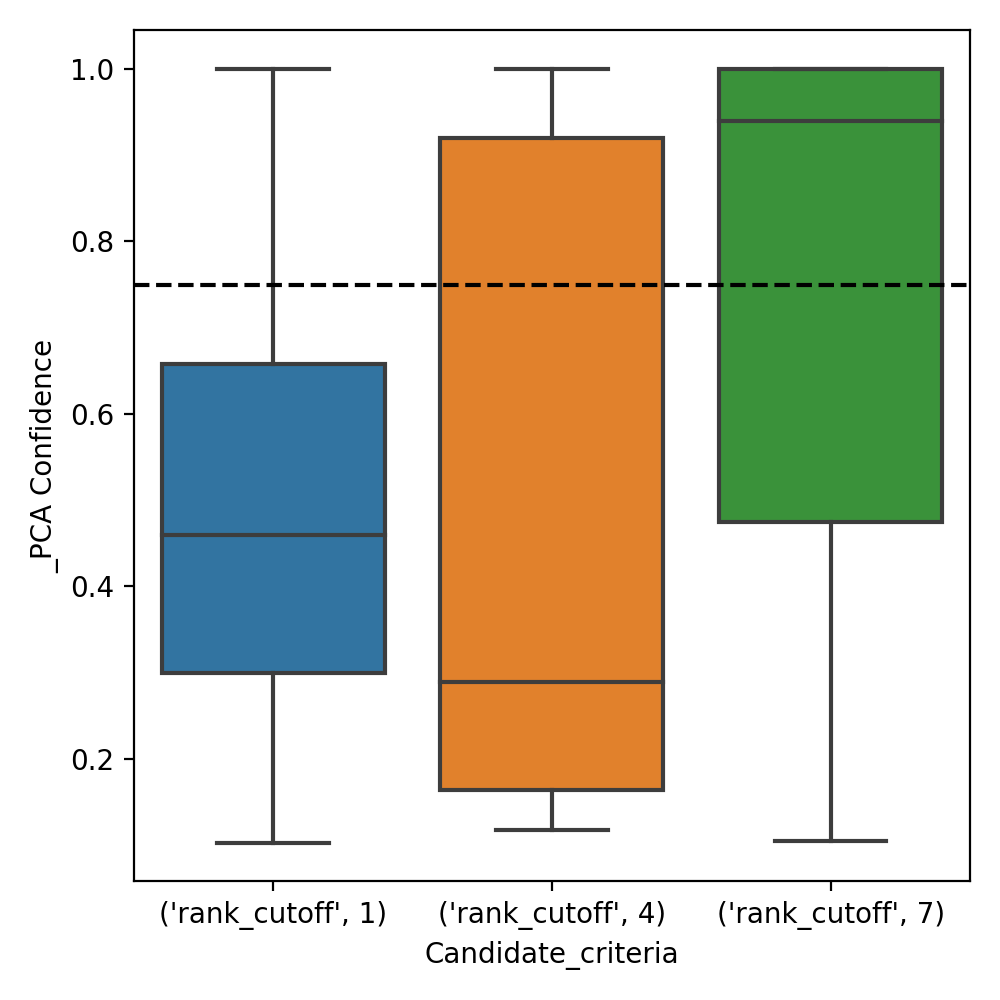
\includegraphics[width=1\linewidth]{figures/results/ranks/_PCA-rank_wn18rr.png}
  \caption{Extended KG}
  \label{fig:_PCA_rank_wn18rr_boxplot_sub}
\end{subfigure}
\caption{Distribution of PCA confidence of mined rules over rank cutoff values. PCA confidence scores are calculated on the original WN18RR and the extended WN18RR from which the rules are mined. The dashed line represents the median PCA confidence of the rules mined from the original WN18RR KG.}
\label{fig:PCA_rank_wn18rr_boxplot}
\end{figure}

\begin{figure}[h]
\centering
\begin{subfigure}{.5\textwidth}
  \centering
  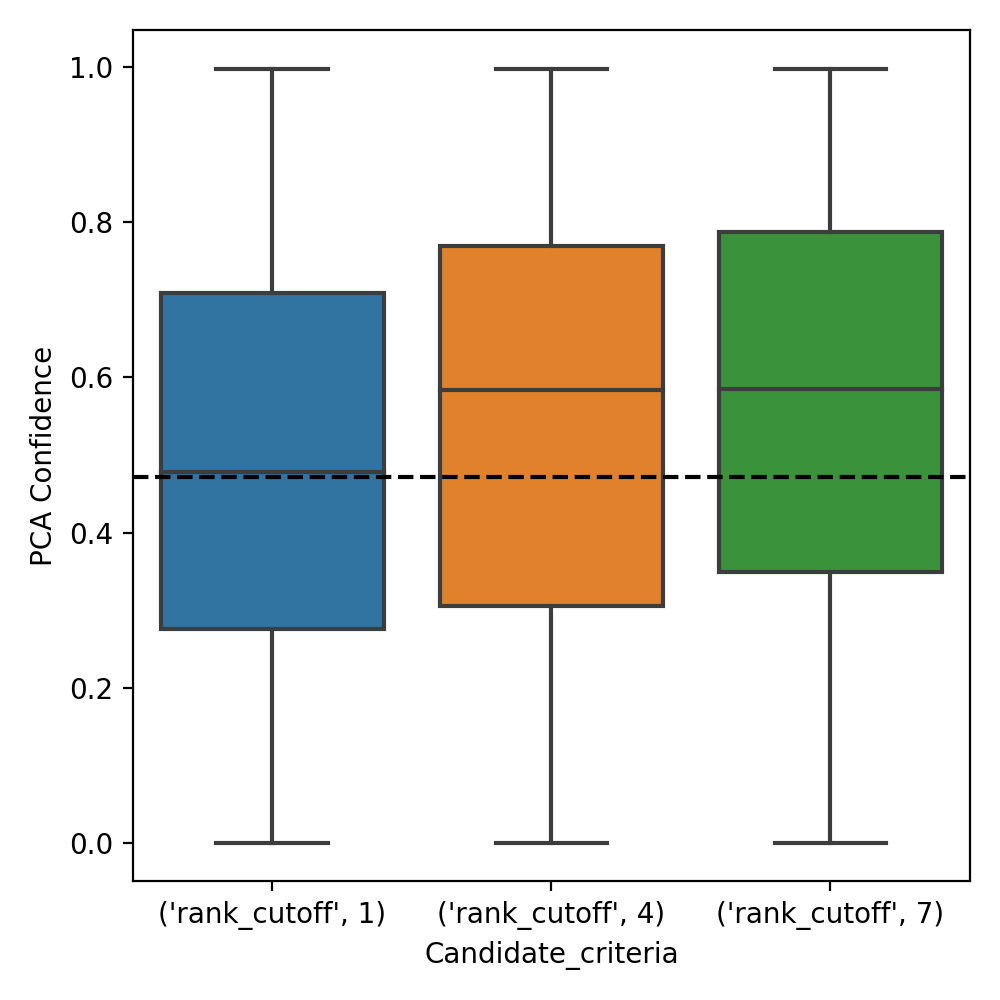
\includegraphics[width=1\linewidth]{figures/results/ranks/PCA-rank_family.png}
  \caption{Original KG}
  \label{fig:models_rank_boxplot_sub}
\end{subfigure}%
\begin{subfigure}{.5\textwidth}
  \centering
  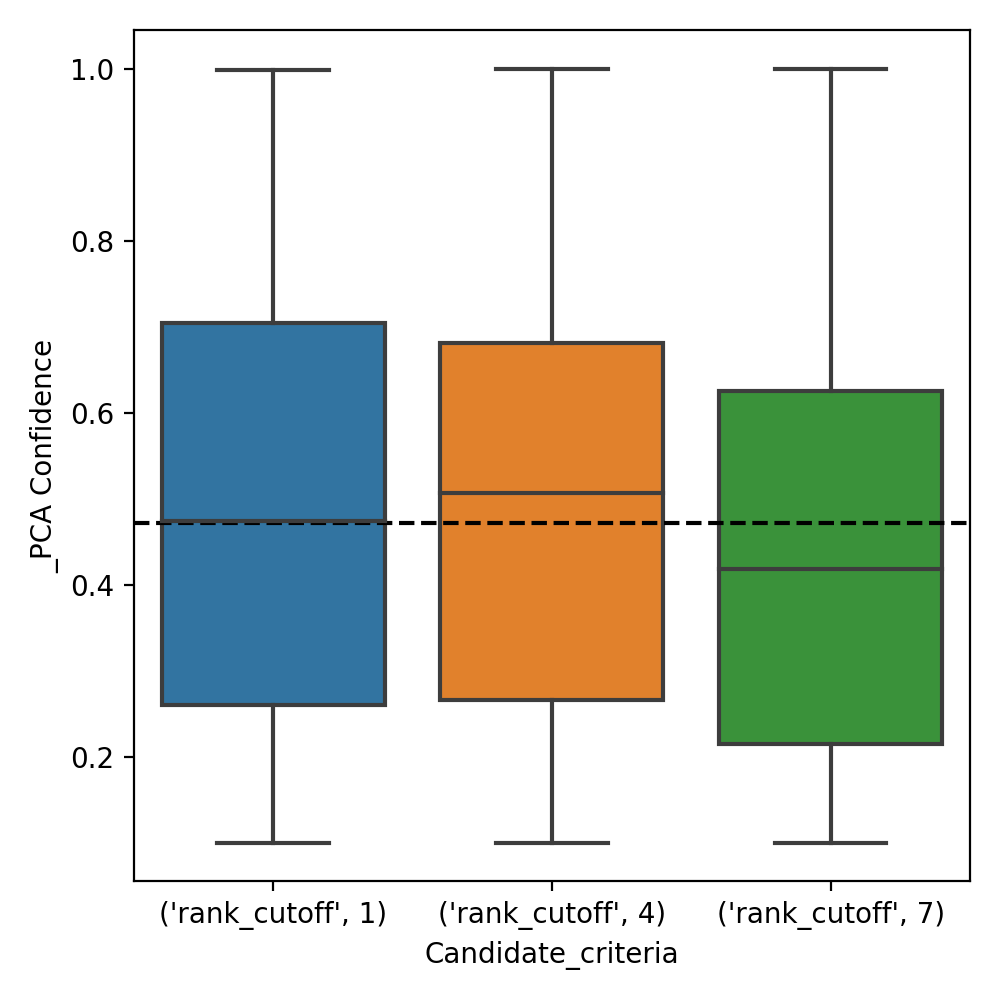
\includegraphics[width=1\linewidth]{figures/results/ranks/_PCA-rank_family.png}
  \caption{Extended KG}
  \label{fig:_PCA_rank_family_boxplot_sub}
\end{subfigure}
\caption{Distribution of PCA confidence of mined rules by rank cutoff values. PCA confidence scores are calculated on the original family KG and the extended family KG from which the rules are mined. The dashed line represents the median PCA confidence of the rules mined from the original family KG.}
\label{fig:PCA_entity_family_boxplot}
\end{figure}







\begin{figure*}[h]
        \centering
        \begin{subfigure}[b]{0.49\textwidth}
            \centering
            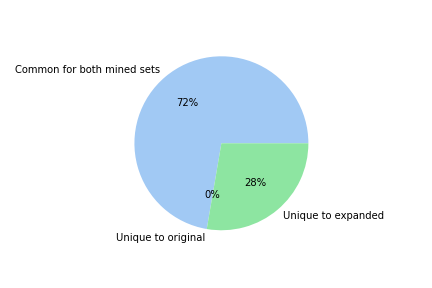
\includegraphics[width=\textwidth]{figures/results/ranks/pie_charts/('rank_cutoff', 1)_family.png}
            \caption[]%
            {{\small Rank 1}}    
            \label{fig:rank_1_pie_family}
        \end{subfigure}
        \hfill
        \begin{subfigure}[b]{0.49\textwidth}  
            \centering 
            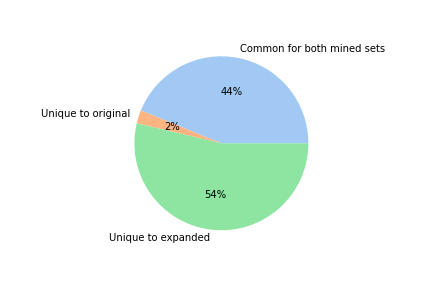
\includegraphics[width=\textwidth]{figures/results/ranks/pie_charts/('rank_cutoff', 4)_family.png}
            \caption[]%
            {{\small Rank 4}}    
            \label{fig:rank_4_pie_family}
        \end{subfigure}
        \vskip\baselineskip
        \begin{subfigure}[b]{0.49\textwidth}   
            \centering 
            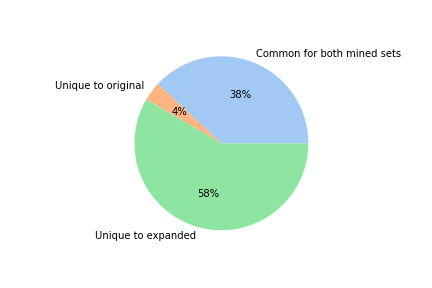
\includegraphics[width=\textwidth]{figures/results/ranks/pie_charts/('rank_cutoff', 7)_family.png}
            \caption[]%
            {{\small Rank 7}}    
            \label{fig:rank_1_pie_family}
        \end{subfigure}
        \hfill
        \caption[]
        {\small Distribution of all the rules mined over KG rank cutoff values. KG: family KG.} 
        \label{fig:rank_pies_family}
    \end{figure*}
    
    
    \begin{figure*}[h]
        \centering
        \begin{subfigure}[b]{0.49\textwidth}
            \centering
            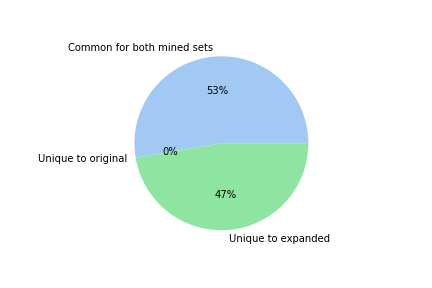
\includegraphics[width=\textwidth]{figures/results/ranks/pie_charts/('rank_cutoff', 1)_wn18rr.png}
            \caption[]%
            {{\small Rank 1}}    
            \label{fig:rank_1_pie_wn18rr}
        \end{subfigure}
        \hfill
        \begin{subfigure}[b]{0.49\textwidth}  
            \centering 
            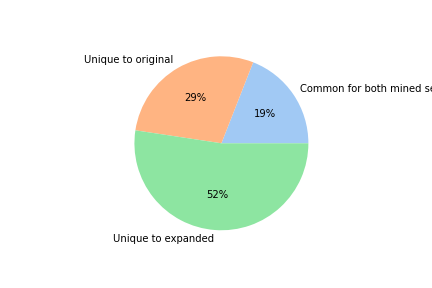
\includegraphics[width=\textwidth]{figures/results/ranks/pie_charts/('rank_cutoff', 4)_wn18rr.png}
            \caption[]%
            {{\small Rank 4}}    
            \label{fig:rank_4_pie_wn18rr}
        \end{subfigure}
        \vskip\baselineskip
        \begin{subfigure}[b]{0.49\textwidth}   
            \centering 
            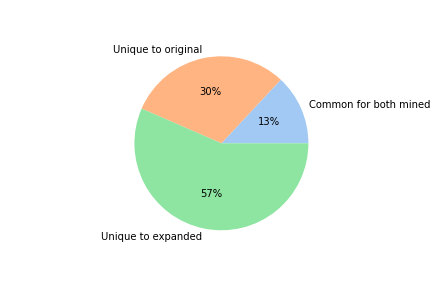
\includegraphics[width=\textwidth]{figures/results/ranks/pie_charts/('rank_cutoff', 7)_wn18rr.png}
            \caption[]%
            {{\small Rank 7}}    
            \label{fig:rank_7_pie_wn18rr}
        \end{subfigure}
        \hfill
        \caption[ ]
        {\small Distribution of all the rules mined over rank cutoff values. KG: WN18RR.} 
        \label{fig:rank_pies_wn18rr}
    \end{figure*}